\section{Пример установки ownCloud Server в Debian GNU/Linux} \label{pril:c}

После успешного входа в систему, в первую очередь необходимо получить права суперпользователя\footnote{Пароль пользователя не отображается на экране во время набора}:
\begin{lstlisting}
student@student-name:~$ su -
Password: toor
\end{lstlisting}

Добавление репозитория и ключа для ownCloud Server:
\begin{lstlisting}
root@student-name:~# wget -nv https://goo.gl/mmV2ga -O Release.key
root@student-name:~# apt-key add - < Release.key
OK
root@student-name:~# echo deb http://download.owncloud.org \
> /download/repositories/stable/Debian_8.0/ / > \
> /etc/apt/sources.list.d/owncloud.list
\end{lstlisting}

После добавления репозитория необходимо обновить список доступного в репозиториях ПО и запустить установку ownCloud Server (во время установки MySQL, установщик запросит пароль суперпользователя MySQL, он не обязательно должен совпадать с паролем пользователя root):
\begin{lstlisting}
root@student-name:~# apt-get update
root@student-name:~# apt-get install owncloud owncloud-files
...
New password for the MySQL "root" user: toor-mysql
Repeat password for the MySQL "root" user: toor-mysql
\end{lstlisting}

После того, как установщик скачал и установил все необходимые пакеты, можно проверить корректность установки (рис.~\ref{pic:first-own}), зайдя по адресу \texttt{http://192.168.0.102/owncloud/}, \\
где \texttt{192.168.0.102} "--- IP-адрес сервера (виртуальной машины).

\begin{figure}[ht]
    \centering
	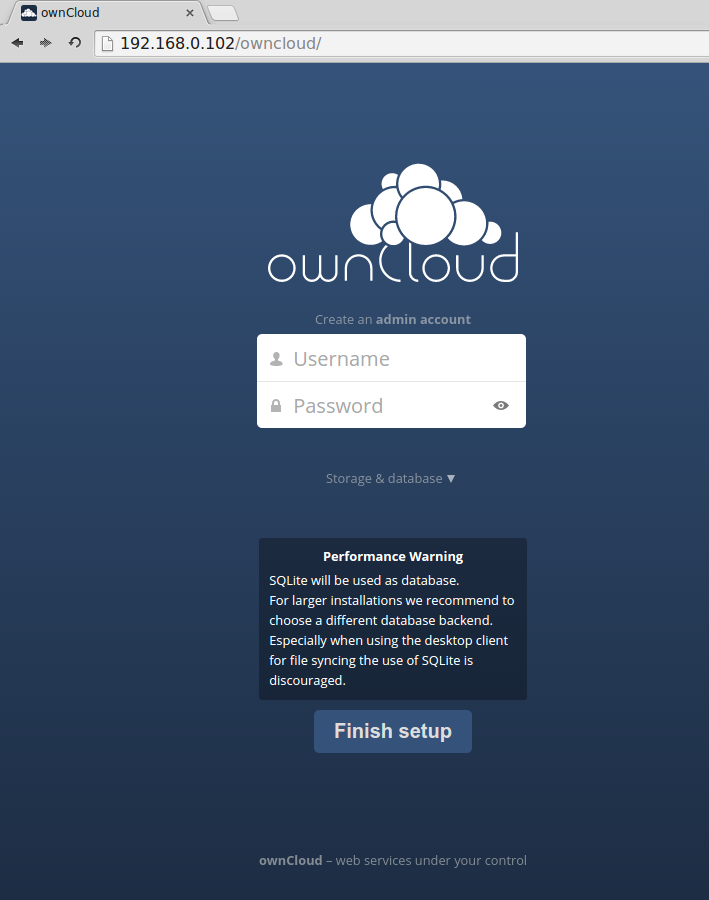
\includegraphics[width=0.7\linewidth]{Screenshot-owncloud}
	\caption{Первый запуск приложения}\label{pic:first-own}
\end{figure}

Приложение предлагает использовать базу данных SQLite по умолчанию, мы же будем использовать MySQL:
\begin{lstlisting}
root@student-name:~# mysql -uroot -ptoor-mysql
mysql> CREATE DATABASE owncloud_DB;
mysql> CREATE USER "owncloud-web"@"localhost" \
    -> IDENTIFIED BY "owncloud-passwd";
mysql> GRANT ALL PRIVILEGES ON owncloud_DB.* \
    -> TO "owncloud-web"@"localhost";
mysql> FLUSH PRIVILEGES;
mysql> quit
\end{lstlisting}

После создания базы данных, необходимо обновить страницу приложения, настроить параметры базы данных и установить данные аккаунта администратора ownCloud (рис.~\ref{pic:db-own}).

\begin{figure}[ht]
    \centering
	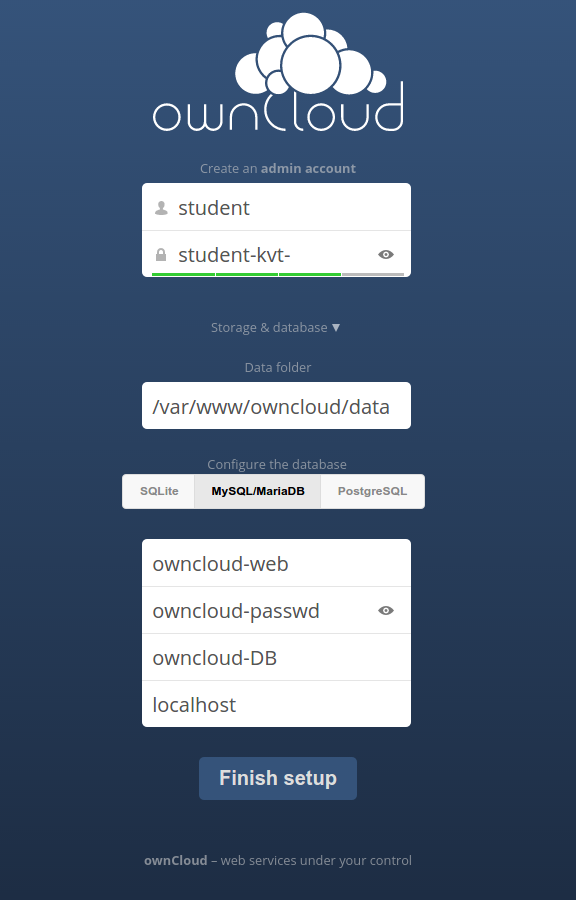
\includegraphics[width=0.8\linewidth]{Screenshot-2-owncloud}
	\caption{Параметры БД и аккаунта администратора}\label{pic:db-own}
\end{figure}

После нажатия клавиши <<Finish Setup>> база данных и пользовательские настройки успешно подключаются к ownCloud (рис.~\ref{pic:interface-own}).

\begin{figure}[ht]
    \centering
	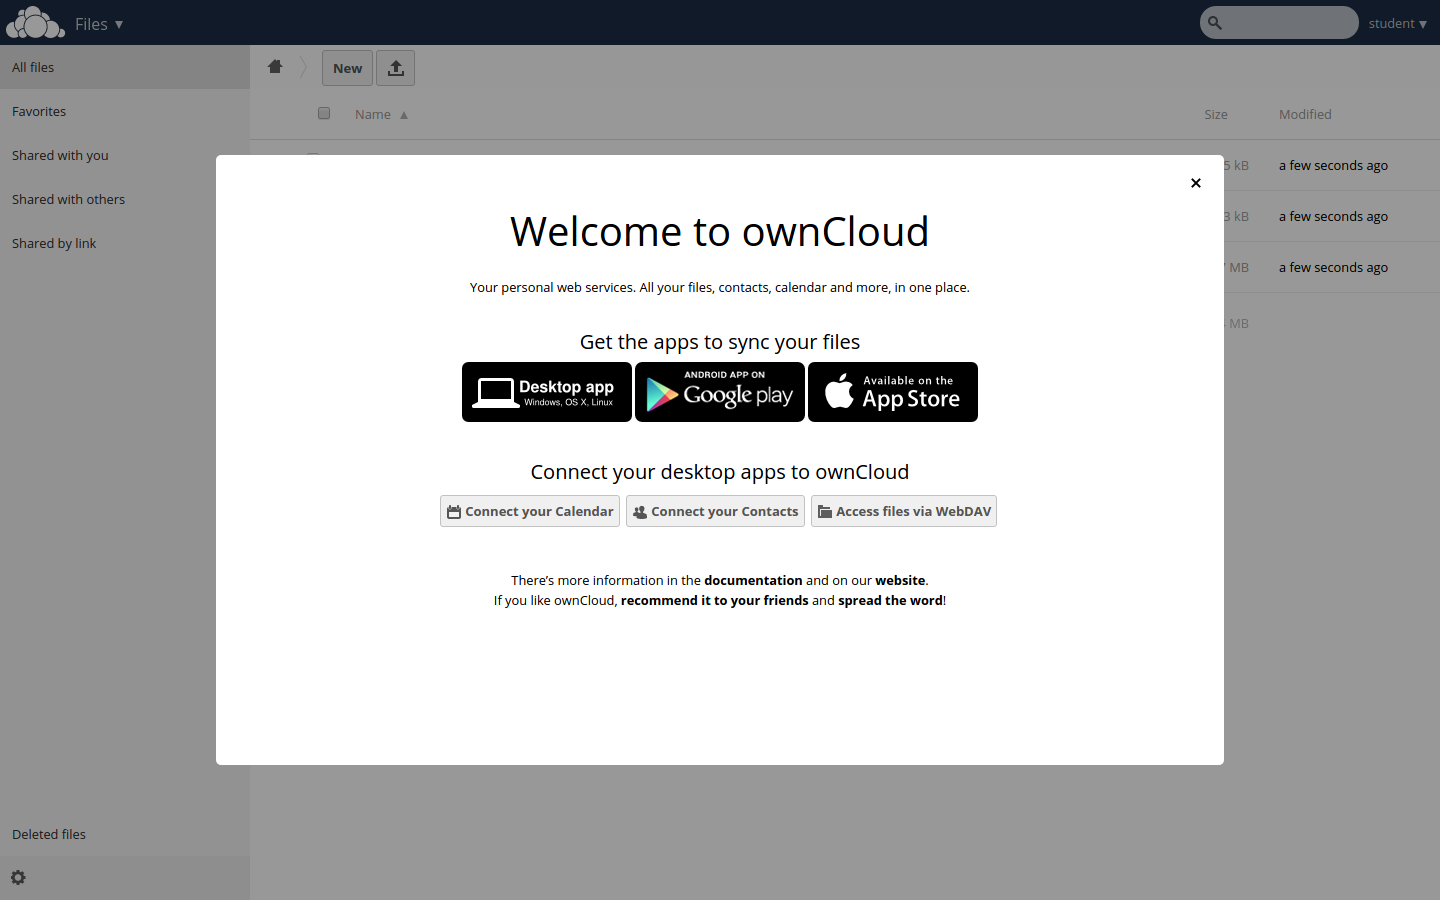
\includegraphics[width=\linewidth]{Screenshot-3-owncloud}
	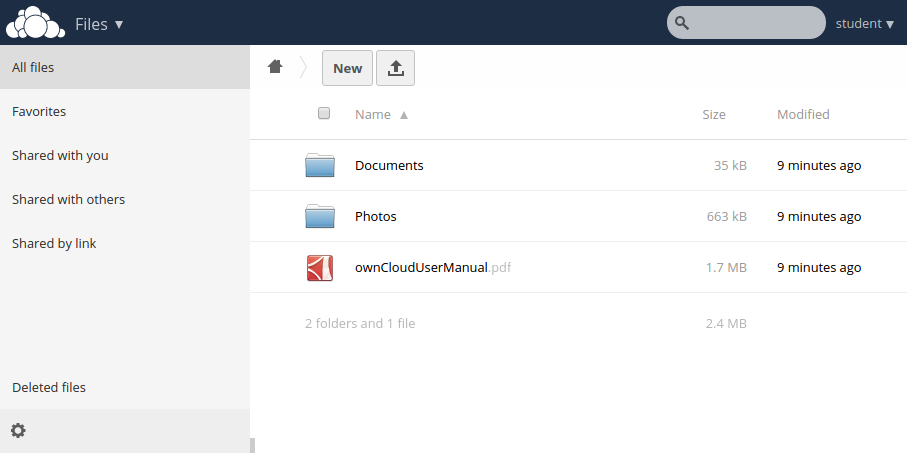
\includegraphics[width=\linewidth]{Screenshot-4-owncloud}
	\caption{Первый вход в ownCloud и интерфейс приложения}\label{pic:interface-own}
\end{figure}

\clearpage
